\chapter{}\label{ch:aufg3}
Im folgenden sollen wir nun den Schrittmotor unter den Gegebenheiten betrachten:
\begin{center}
	$ M_{H} = 1.17Nm \hspace{1cm} Z_{P} = 50 \hspace{1cm} m = 2 $
\end{center}

\section{}\label{sec:3a}
Es soll der mechanische Winkel $ \lambda_{mL} $ bestimmt werden, um den der Schrittmotor in der Ruhelage ausgerenkt wird. Als Grundlage für die Berechnung ziehen wir folgende Formel heran:
\begin{equation}
	M_{L} = M_{H}sin(\lambda_{S}-\lambda_{L}) \hspace{1.5cm} mit~\lambda_{S} = 0
\end{equation}
Diese Formel stellen wir nach $ \lambda_{L} $ um und setzen die gegeneben Werte ein. Wir erhalten den zu bestimmenden Lastwinkel.

\begin{equation}
	\lambda_{mL} = \frac{\lambda_{L}}{Z_{P}}
\end{equation}
Unter der Berücksichtigung der gegebenen Polpaarzahl können nun den mechanischen Winkel $ \lambda_{mL} $ bestimmen.

\section{}\label{sec:3b}
Es soll anhand des Diagramm nun graphisch der Winkel $ \lambda_{mL} $ ermittelt werden, um den der Schrittmotor in der Ruhelage $ \lambda_{m} = 0 $ ausgelenkt wird. Des weiteren soll die Abszisse noch mit dem passenden Winkel beschriftet werden. Mit dem Verhältnis $ \frac{M_{L}}{M_{H}} $ können wir den Lastwinkel $ \lambda_{L} $ bestimmen. Diesen können wir dann anschließend graphisch auswerten.
\begin{figure}[h]
	\centering
	% This file was created by matlab2tikz.
%
%The latest updates can be retrieved from
%  http://www.mathworks.com/matlabcentral/fileexchange/22022-matlab2tikz-matlab2tikz
%where you can also make suggestions and rate matlab2tikz.
%
\definecolor{mycolor1}{rgb}{0.00000,0.44700,0.74100}%
\definecolor{mycolor2}{rgb}{0.85000,0.32500,0.09800}
%
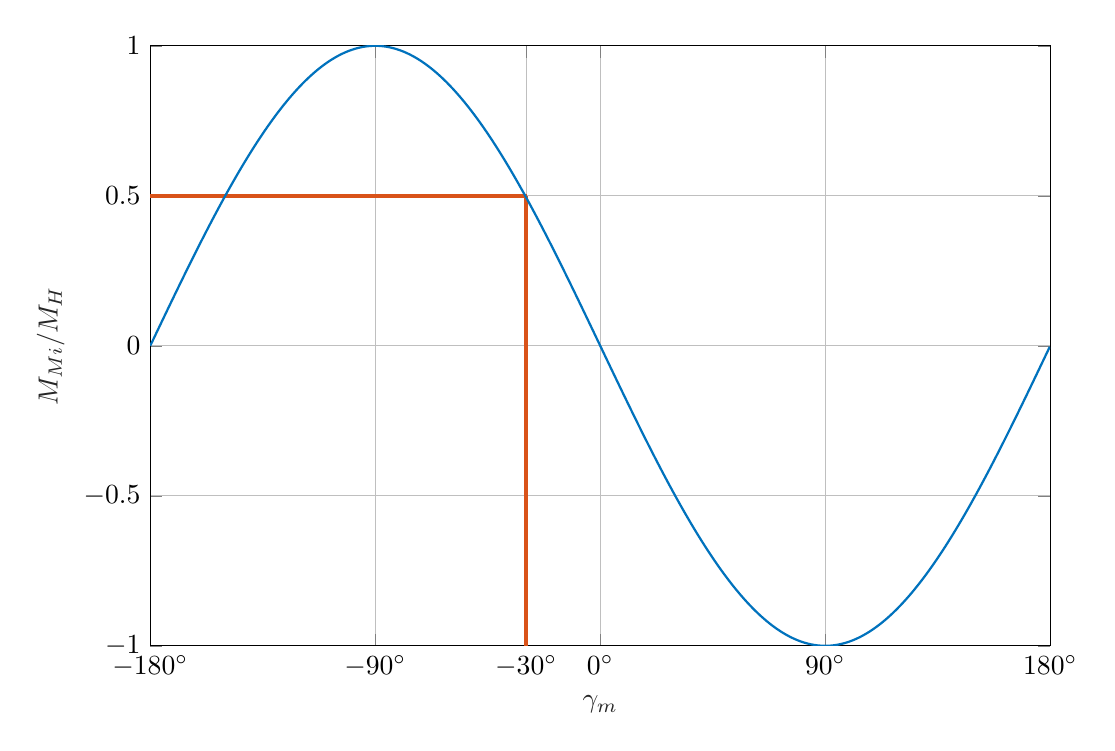
\begin{tikzpicture}

\begin{axis}[%
width=4.5in,
height=3in,
scale only axis,
xmin=-3.14159265358979,
xmax=3.14159265358979,
xtick={-3.14159265358979,-1.5707963267949,-0.517,0,1.5707963267949,3.14159265358979},
xticklabels={{$ -180^{\circ} $},{$ -90^{\circ} $},{$ -30^{\circ} $},{$ 0^{\circ} $},{$ 90^{\circ} $},{$ 180^{\circ} $}},
xlabel style={font=\color{white!15!black}},
xlabel={$\gamma_{m}$},
ymin=-1,
ymax=1,
ytick={  -1, -0.5,    0,  0.5,    1},
ylabel style={font=\color{white!15!black}},
ylabel={$ M_{Mi}/M_{H} $},
axis background/.style={fill=white},
xmajorgrids,
ymajorgrids,
every axis plot/.append style={thick}
]

\draw [ultra thick, mycolor2] (0in,2.25in) -- (1.884in,2.25in);
\draw [ultra thick, mycolor2] (1.88in, 2.25in) -- (1.88in, 0in);

\addplot [color=mycolor1]
  table[row sep=crcr]{%
-3.14159265358979	1.22464679914735e-16\\
-3.13159265358979	0.00999983333416657\\
-3.12159265358979	0.0199986666933332\\
-3.11159265358979	0.0299955002024956\\
-3.10159265358979	0.0399893341866343\\
-3.09159265358979	0.0499791692706783\\
-3.08159265358979	0.0599640064794448\\
-3.07159265358979	0.0699428473375327\\
-3.06159265358979	0.0799146939691729\\
-3.05159265358979	0.089878549198011\\
-3.04159265358979	0.0998334166468284\\
-3.03159265358979	0.109778300837175\\
-3.02159265358979	0.11971220728892\\
-3.01159265358979	0.129634142619695\\
-3.00159265358979	0.139543114644237\\
-2.99159265358979	0.149438132473599\\
-2.98159265358979	0.159318206614246\\
-2.97159265358979	0.169182349066996\\
-2.96159265358979	0.179029573425824\\
-2.95159265358979	0.188858894976501\\
-2.94159265358979	0.198669330795062\\
-2.93159265358979	0.2084598998461\\
-2.92159265358979	0.21822962308087\\
-2.91159265358979	0.227977523535188\\
-2.90159265358979	0.237702626427135\\
-2.89159265358979	0.247403959254523\\
-2.88159265358979	0.257080551892155\\
-2.87159265358979	0.266731436688831\\
-2.86159265358979	0.276355648564114\\
-2.85159265358979	0.285952225104836\\
-2.84159265358979	0.29552020666134\\
-2.83159265358979	0.305058636443444\\
-2.82159265358979	0.314566560616118\\
-2.81159265358979	0.324043028394869\\
-2.80159265358979	0.333487092140814\\
-2.79159265358979	0.342897807455452\\
-2.78159265358979	0.35227423327509\\
-2.77159265358979	0.361615431964962\\
-2.76159265358979	0.370920469412983\\
-2.75159265358979	0.380188415123162\\
-2.74159265358979	0.389418342308651\\
-2.73159265358979	0.398609327984423\\
-2.72159265358979	0.40776045305957\\
-2.71159265358979	0.416870802429211\\
-2.70159265358979	0.425939465066\\
-2.69159265358979	0.43496553411123\\
-2.68159265358979	0.44394810696552\\
-2.67159265358979	0.452886285379069\\
-2.66159265358979	0.461779175541483\\
-2.65159265358979	0.470625888171158\\
-2.64159265358979	0.479425538604203\\
-2.63159265358979	0.488177246882907\\
-2.62159265358979	0.496880137843737\\
-2.61159265358979	0.505533341204847\\
-2.60159265358979	0.514135991653113\\
-2.59159265358979	0.522687228930659\\
-2.58159265358979	0.531186197920884\\
-2.57159265358979	0.53963204873397\\
-2.56159265358979	0.548023936791874\\
-2.55159265358979	0.556361022912784\\
-2.54159265358979	0.564642473395035\\
-2.53159265358979	0.572867460100481\\
-2.52159265358979	0.581035160537305\\
-2.51159265358979	0.58914475794227\\
-2.50159265358979	0.597195441362392\\
-2.49159265358979	0.60518640573604\\
-2.48159265358979	0.613116851973434\\
-2.47159265358979	0.62098598703656\\
-2.46159265358979	0.628793024018469\\
-2.45159265358979	0.636537182221968\\
-2.44159265358979	0.644217687237691\\
-2.43159265358979	0.651833771021537\\
-2.42159265358979	0.659384671971473\\
-2.41159265358979	0.666869635003698\\
-2.40159265358979	0.674287911628145\\
-2.39159265358979	0.681638760023334\\
-2.38159265358979	0.688921445110551\\
-2.37159265358979	0.696135238627357\\
-2.36159265358979	0.70327941920041\\
-2.35159265358979	0.710353272417608\\
-2.34159265358979	0.717356090899523\\
-2.33159265358979	0.724287174370143\\
-2.32159265358979	0.731145829726896\\
-2.31159265358979	0.737931371109963\\
-2.30159265358979	0.744643119970859\\
-2.29159265358979	0.751280405140293\\
-2.28159265358979	0.757842562895277\\
-2.27159265358979	0.764328937025505\\
-2.26159265358979	0.770738878898969\\
-2.25159265358979	0.777071747526824\\
-2.24159265358979	0.783326909627483\\
-2.23159265358979	0.789503739689951\\
-2.22159265358979	0.795601620036366\\
-2.21159265358979	0.801619940883777\\
-2.20159265358979	0.807558100405114\\
-2.19159265358979	0.813415504789374\\
-2.18159265358979	0.819191568300998\\
-2.17159265358979	0.82488571333845\\
-2.16159265358979	0.83049737049197\\
-2.15159265358979	0.836025978600521\\
-2.14159265358979	0.841470984807897\\
-2.13159265358979	0.846831844618015\\
-2.12159265358979	0.852108021949363\\
-2.11159265358979	0.857298989188604\\
-2.10159265358979	0.862404227243338\\
-2.09159265358979	0.867423225594017\\
-2.08159265358979	0.872355482344986\\
-2.07159265358979	0.877200504274682\\
-2.06159265358979	0.881957806884948\\
-2.05159265358979	0.886626914449487\\
-2.04159265358979	0.891207360061435\\
-2.03159265358979	0.895698685680048\\
-2.02159265358979	0.900100442176505\\
-2.01159265358979	0.904412189378826\\
-2.00159265358979	0.908633496115883\\
-1.99159265358979	0.912763940260521\\
-1.98159265358979	0.916803108771767\\
-1.97159265358979	0.920750597736136\\
-1.96159265358979	0.92460601240802\\
-1.95159265358979	0.928368967249167\\
-1.94159265358979	0.932039085967226\\
-1.93159265358979	0.935616001553386\\
-1.92159265358979	0.939099356319068\\
-1.91159265358979	0.942488801931698\\
-1.90159265358979	0.945783999449539\\
-1.89159265358979	0.948984619355586\\
-1.88159265358979	0.952090341590516\\
-1.87159265358979	0.955100855584692\\
-1.86159265358979	0.958015860289225\\
-1.85159265358979	0.960835064206073\\
-1.84159265358979	0.963558185417193\\
-1.83159265358979	0.966184951612734\\
-1.82159265358979	0.968715100118265\\
-1.81159265358979	0.971148377921045\\
-1.80159265358979	0.973484541695319\\
-1.79159265358979	0.975723357826659\\
-1.78159265358979	0.977864602435316\\
-1.77159265358979	0.979908061398614\\
-1.76159265358979	0.98185353037236\\
-1.75159265358979	0.983700814811277\\
-1.74159265358979	0.98544972998846\\
-1.73159265358979	0.98710010101385\\
-1.72159265358979	0.98865176285172\\
-1.71159265358979	0.990104560337178\\
-1.70159265358979	0.991458348191686\\
-1.69159265358979	0.992712991037588\\
-1.68159265358979	0.993868363411645\\
-1.67159265358979	0.994924349777581\\
-1.66159265358979	0.99588084453764\\
-1.65159265358979	0.996737752043143\\
-1.64159265358979	0.997494986604054\\
-1.63159265358979	0.998152472497548\\
-1.62159265358979	0.998710143975583\\
-1.61159265358979	0.999167945271476\\
-1.60159265358979	0.999525830605479\\
-1.59159265358979	0.999783764189357\\
-1.58159265358979	0.999941720229966\\
-1.57159265358979	0.999999682931835\\
-1.56159265358979	0.99995764649874\\
-1.55159265358979	0.999815615134291\\
-1.54159265358979	0.999573603041505\\
-1.53159265358979	0.999231634421391\\
-1.52159265358979	0.998789743470524\\
-1.51159265358979	0.998247974377632\\
-1.50159265358979	0.997606381319174\\
-1.49159265358979	0.996865028453919\\
-1.48159265358979	0.996023989916537\\
-1.47159265358979	0.99508334981018\\
-1.46159265358979	0.994043202198076\\
-1.45159265358979	0.992903651094118\\
-1.44159265358979	0.991664810452469\\
-1.43159265358979	0.990326804156158\\
-1.42159265358979	0.988889766004701\\
-1.41159265358979	0.987353839700716\\
-1.40159265358979	0.985719178835553\\
-1.39159265358979	0.983985946873937\\
-1.38159265358979	0.982154317137618\\
-1.37159265358979	0.980224472788045\\
-1.36159265358979	0.978196606808045\\
-1.35159265358979	0.976070921982524\\
-1.34159265358979	0.973847630878195\\
-1.33159265358979	0.971526955822315\\
-1.32159265358979	0.969109128880456\\
-1.31159265358979	0.966594391833298\\
-1.30159265358979	0.963982996152448\\
-1.29159265358979	0.9612752029753\\
-1.28159265358979	0.958471283078914\\
-1.27159265358979	0.955571516852944\\
-1.26159265358979	0.952576194271595\\
-1.25159265358979	0.94948561486463\\
-1.24159265358979	0.946300087687414\\
-1.23159265358979	0.94301993129001\\
-1.22159265358979	0.939645473685325\\
-1.21159265358979	0.936177052316306\\
-1.20159265358979	0.9326150140222\\
-1.19159265358979	0.928959715003869\\
-1.18159265358979	0.925211520788168\\
-1.17159265358979	0.921370806191395\\
-1.16159265358979	0.91743795528181\\
-1.15159265358979	0.913413361341225\\
-1.14159265358979	0.909297426825682\\
-1.13159265358979	0.905090563325201\\
-1.12159265358979	0.900793191522627\\
-1.11159265358979	0.89640574115156\\
-1.10159265358979	0.89192865095338\\
-1.09159265358979	0.887362368633375\\
-1.08159265358979	0.882707350815974\\
-1.07159265358979	0.877964062999078\\
-1.06159265358979	0.873132979507516\\
-1.05159265358979	0.868214583445613\\
-1.04159265358979	0.863209366648874\\
-1.03159265358979	0.858117829634809\\
-1.02159265358979	0.852940481552876\\
-1.01159265358979	0.84767784013357\\
-1.00159265358979	0.842330431636646\\
-0.991592653589793	0.836898790798498\\
-0.981592653589793	0.831383460778683\\
-0.971592653589793	0.825784993105608\\
-0.961592653589793	0.820103947621374\\
-0.951592653589793	0.814340892425796\\
-0.941592653589793	0.80849640381959\\
-0.931592653589793	0.802571066246747\\
-0.921592653589793	0.796565472236086\\
-0.911592653589793	0.790480222342005\\
-0.901592653589793	0.78431592508442\\
-0.891592653589793	0.778073196887921\\
-0.881592653589793	0.771752662020126\\
-0.871592653589793	0.765354952529253\\
-0.861592653589793	0.758880708180922\\
-0.851592653589793	0.752330576394171\\
-0.841592653589793	0.74570521217672\\
-0.831592653589793	0.739005278059471\\
-0.821592653589793	0.732231444030251\\
-0.811592653589793	0.725384387466819\\
-0.801592653589793	0.718464793069126\\
-0.791592653589793	0.711473352790844\\
-0.781592653589793	0.704410765770176\\
-0.771592653589793	0.697277738259938\\
-0.761592653589793	0.690074983556936\\
-0.751592653589793	0.68280322193064\\
-0.741592653589793	0.675463180551151\\
-0.731592653589793	0.668055593416491\\
-0.721592653589793	0.660581201279201\\
-0.711592653589793	0.653040751572265\\
-0.701592653589793	0.645434998334371\\
-0.691592653589793	0.637764702134504\\
-0.681592653589793	0.630030629995892\\
-0.671592653589793	0.622233555319305\\
-0.661592653589793	0.614374257805712\\
-0.651592653589793	0.606453523378315\\
-0.641592653589793	0.598472144103956\\
-0.631592653589793	0.590430918113913\\
-0.621592653589793	0.582330649524082\\
-0.611592653589793	0.574172148354572\\
-0.601592653589793	0.565956230448703\\
-0.591592653589793	0.557683717391417\\
-0.581592653589793	0.549355436427127\\
-0.571592653589793	0.540972220376988\\
-0.561592653589793	0.532534907555621\\
-0.551592653589793	0.524044341687276\\
-0.541592653589793	0.515501371821464\\
-0.531592653589793	0.506906852248053\\
-0.521592653589793	0.498261642411838\\
-0.511592653589793	0.489566606826599\\
-0.501592653589793	0.480822614988648\\
-0.491592653589793	0.472030541289883\\
-0.481592653589793	0.463191264930345\\
-0.471592653589793	0.454305669830306\\
-0.461592653589793	0.445374644541871\\
-0.451592653589793	0.436399082160126\\
-0.441592653589793	0.42737988023383\\
-0.431592653589793	0.418317940675659\\
-0.421592653589793	0.409214169672017\\
-0.411592653589793	0.400069477592419\\
-0.401592653589793	0.390884778898452\\
-0.391592653589793	0.381660992052332\\
-0.381592653589793	0.372399039425055\\
-0.371592653589793	0.363099847204168\\
-0.361592653589793	0.353764345301143\\
-0.351592653589793	0.34439346725839\\
-0.341592653589793	0.334988150155905\\
-0.331592653589793	0.32554933451756\\
-0.321592653589793	0.316077964217054\\
-0.311592653589793	0.306574986383523\\
-0.301592653589793	0.297041351306832\\
-0.291592653589793	0.287478012342544\\
-0.281592653589793	0.277885925816587\\
-0.271592653589793	0.268266050929618\\
-0.261592653589793	0.258619349661111\\
-0.251592653589793	0.248946786673152\\
-0.241592653589793	0.239249329213982\\
-0.231592653589793	0.229527947021264\\
-0.221592653589793	0.219783612225117\\
-0.211592653589793	0.210017299250899\\
-0.201592653589793	0.20022998472177\\
-0.191592653589793	0.190422647361027\\
-0.181592653589793	0.180596267894233\\
-0.171592653589793	0.170751828951145\\
-0.161592653589793	0.160890314967456\\
-0.151592653589793	0.151012712086344\\
-0.141592653589793	0.141120008059867\\
-0.131592653589793	0.131213192150184\\
-0.121592653589793	0.12129325503063\\
-0.111592653589793	0.111361188686649\\
-0.101592653589793	0.101417986316602\\
-0.0915926535897928	0.0914646422324366\\
-0.0815926535897931	0.081502151760269\\
-0.0715926535897928	0.0715315111408431\\
-0.061592653589793	0.061553717429913\\
-0.0515926535897933	0.0515697683985345\\
-0.041592653589793	0.0415806624332904\\
-0.0315926535897932	0.0315873984364538\\
-0.021592653589793	0.0215909757260958\\
-0.0115926535897932	0.0115923939361582\\
-0.00159265358979299	0.00159265291648671\\
0.00840734641020724	-0.00840724736714918\\
0.018407346410207	-0.0184063069330539\\
0.0284073464102073	-0.0284035258836044\\
0.038407346410207	-0.0383979045052355\\
0.0484073464102073	-0.0483884433684147\\
0.0584073464102071	-0.0583741434275802\\
0.0684073464102068	-0.0683540061210479\\
0.0784073464102071	-0.0783270334708654\\
0.0884073464102069	-0.0882922281826077\\
0.0984073464102071	-0.0982485937451088\\
0.108407346410207	-0.108195134530108\\
0.118407346410207	-0.118130855891818\\
0.128407346410207	-0.12805476426638\\
0.138407346410207	-0.137965867271227\\
0.148407346410207	-0.147863173804319\\
0.158407346410207	-0.157745694143249\\
0.168407346410207	-0.167612440044218\\
0.178407346410207	-0.177462424840861\\
0.188407346410207	-0.187294663542903\\
0.198407346410207	-0.19710817293467\\
0.208407346410207	-0.2069019716734\\
0.218407346410207	-0.21667508038738\\
0.228407346410207	-0.226426521773883\\
0.238407346410207	-0.236155320696898\\
0.248407346410207	-0.245860504284637\\
0.258407346410207	-0.255541102026832\\
0.268407346410207	-0.265196145871774\\
0.278407346410207	-0.274824670323125\\
0.288407346410207	-0.284425712536463\\
0.298407346410207	-0.293998312415568\\
0.308407346410207	-0.303541512708429\\
0.318407346410207	-0.313054359102971\\
0.328407346410207	-0.322535900322479\\
0.338407346410207	-0.331985188220734\\
0.348407346410207	-0.341401277876821\\
0.358407346410207	-0.35078322768962\\
0.368407346410207	-0.360130099471969\\
0.378407346410207	-0.369440958544477\\
0.388407346410207	-0.378714873828998\\
0.398407346410207	-0.38795091794173\\
0.408407346410207	-0.39714816728596\\
0.418407346410207	-0.406305702144417\\
0.428407346410207	-0.415422606771246\\
0.438407346410207	-0.424497969483583\\
0.448407346410207	-0.433530882752718\\
0.458407346410207	-0.442520443294853\\
0.468407346410207	-0.451465752161424\\
0.478407346410207	-0.460365914828998\\
0.488407346410207	-0.469220041288728\\
0.498407346410207	-0.478027246135343\\
0.508407346410207	-0.4867866486557\\
0.518407346410207	-0.495497372916845\\
0.528407346410207	-0.504158547853612\\
0.538407346410207	-0.512769307355724\\
0.548407346410207	-0.521328790354407\\
0.558407346410207	-0.529836140908494\\
0.568407346410207	-0.538290508290018\\
0.578407346410207	-0.546691047069287\\
0.588407346410207	-0.555036917199424\\
0.598407346410207	-0.56332728410037\\
0.608407346410207	-0.571561318742344\\
0.618407346410207	-0.579738197728743\\
0.628407346410207	-0.587857103378483\\
0.638407346410207	-0.595917223807764\\
0.648407346410207	-0.603917753011261\\
0.658407346410207	-0.611857890942719\\
0.668407346410207	-0.619736843594963\\
0.678407346410207	-0.627553823079294\\
0.688407346410207	-0.635308047704276\\
0.698407346410207	-0.642998742053909\\
0.708407346410207	-0.650625137065167\\
0.718407346410207	-0.658186470104905\\
0.728407346410207	-0.665681985046119\\
0.738407346410207	-0.673110932343562\\
0.748407346410207	-0.680472569108694\\
0.758407346410207	-0.687766159183974\\
0.768407346410207	-0.694990973216472\\
0.778407346410207	-0.702146288730806\\
0.788407346410207	-0.709231390201386\\
0.798407346410207	-0.716245569123971\\
0.808407346410207	-0.723188124086512\\
0.818407346410207	-0.7300583608393\\
0.828407346410207	-0.736855592364383\\
0.838407346410207	-0.743579138944275\\
0.848407346410207	-0.750228328229919\\
0.858407346410207	-0.756802495307928\\
0.868407346410207	-0.763300982767074\\
0.878407346410207	-0.769723140764024\\
0.888407346410207	-0.776068327088332\\
0.898407346410207	-0.782335907226653\\
0.908407346410207	-0.788525254426195\\
0.918407346410207	-0.794635749757397\\
0.928407346410207	-0.800666782175818\\
0.938407346410207	-0.806617748583241\\
0.948407346410207	-0.812488053887985\\
0.958407346410207	-0.818277111064411\\
0.968407346410207	-0.823984341211626\\
0.978407346410207	-0.829609173611371\\
0.988407346410207	-0.835151045785094\\
0.998407346410207	-0.840609403550195\\
1.00840734641021	-0.845983701075447\\
1.01840734641021	-0.851273400935575\\
1.02840734641021	-0.856477974165001\\
1.03840734641021	-0.861596900310741\\
1.04840734641021	-0.866629667484444\\
1.05840734641021	-0.871575772413588\\
1.06840734641021	-0.876434720491802\\
1.07840734641021	-0.881206025828326\\
1.08840734641021	-0.885889211296603\\
1.09840734641021	-0.890483808581989\\
1.10840734641021	-0.894989358228584\\
1.11840734641021	-0.899405409685178\\
1.12840734641021	-0.903731521350306\\
1.13840734641021	-0.907967260616405\\
1.14840734641021	-0.91211220391308\\
1.15840734641021	-0.916165936749455\\
1.16840734641021	-0.920128053755624\\
1.17840734641021	-0.923998158723188\\
1.18840734641021	-0.927775864644876\\
1.19840734641021	-0.931460793753243\\
1.20840734641021	-0.935052577558449\\
1.21840734641021	-0.938550856885108\\
1.22840734641021	-0.941955281908201\\
1.23840734641021	-0.945265512188063\\
1.24840734641021	-0.948481216704426\\
1.25840734641021	-0.951602073889516\\
1.26840734641021	-0.954627771660216\\
1.27840734641021	-0.957558007449271\\
1.28840734641021	-0.960392488235543\\
1.29840734641021	-0.963130930573317\\
1.30840734641021	-0.965773060620639\\
1.31840734641021	-0.968318614166707\\
1.32840734641021	-0.970767336658288\\
1.33840734641021	-0.973118983225174\\
1.34840734641021	-0.975373318704666\\
1.35840734641021	-0.977530117665097\\
1.36840734641021	-0.979589164428367\\
1.37840734641021	-0.981550253091516\\
1.38840734641021	-0.983413187547311\\
1.39840734641021	-0.985177781503859\\
1.40840734641021	-0.986843858503237\\
1.41840734641021	-0.988411251939131\\
1.42840734641021	-0.989879805073504\\
1.43840734641021	-0.991249371052267\\
1.44840734641021	-0.992519812919963\\
1.45840734641021	-0.993691003633465\\
1.46840734641021	-0.994762826074676\\
1.47840734641021	-0.995735173062245\\
1.48840734641021	-0.996607947362286\\
1.49840734641021	-0.997381061698093\\
1.50840734641021	-0.998054438758879\\
1.51840734641021	-0.998628011207499\\
1.52840734641021	-0.999101721687185\\
1.53840734641021	-0.999475522827284\\
1.54840734641021	-0.999749377247994\\
1.55840734641021	-0.999923257564101\\
1.56840734641021	-0.999997146387718\\
1.57840734641021	-0.999971036330024\\
1.58840734641021	-0.999844930002004\\
1.59840734641021	-0.999618840014185\\
1.60840734641021	-0.999292788975378\\
1.61840734641021	-0.998866809490414\\
1.62840734641021	-0.998340944156888\\
1.63840734641021	-0.997715245560893\\
1.64840734641021	-0.99698977627177\\
1.65840734641021	-0.996164608835841\\
1.66840734641021	-0.995239825769163\\
1.67840734641021	-0.994215519549271\\
1.68840734641021	-0.993091792605935\\
1.69840734641021	-0.991868757310913\\
1.70840734641021	-0.990546535966713\\
1.71840734641021	-0.98912526079437\\
1.72840734641021	-0.987605073920215\\
1.73840734641021	-0.98598612736167\\
1.74840734641021	-0.984268583012041\\
1.75840734641021	-0.982452612624332\\
1.76840734641021	-0.980538397794069\\
1.77840734641021	-0.978526129941138\\
1.78840734641021	-0.97641601029065\\
1.79840734641021	-0.974208249852809\\
1.80840734641021	-0.971903069401821\\
1.81840734641021	-0.969500699453809\\
1.82840734641021	-0.967001380243766\\
1.83840734641021	-0.96440536170153\\
1.84840734641021	-0.961712903426793\\
1.85840734641021	-0.958924274663138\\
1.86840734641021	-0.956039754271118\\
1.87840734641021	-0.953059630700367\\
1.88840734641021	-0.949984201960761\\
1.89840734641021	-0.946813775592609\\
1.90840734641021	-0.943548668635906\\
1.91840734641021	-0.940189207598628\\
1.92840734641021	-0.936735728424079\\
1.93840734641021	-0.933188576457297\\
1.94840734641021	-0.929548106410525\\
1.95840734641021	-0.925814682327732\\
1.96840734641021	-0.921988677548216\\
1.97840734641021	-0.918070474669267\\
1.98840734641021	-0.914060465507907\\
1.99840734641021	-0.90995905106171\\
2.00840734641021	-0.905766641468704\\
2.01840734641021	-0.901483655966355\\
2.02840734641021	-0.897110522849642\\
2.03840734641021	-0.892647679428234\\
2.04840734641021	-0.888095571982754\\
2.05840734641021	-0.883454655720153\\
2.06840734641021	-0.87872539472819\\
2.07840734641021	-0.873908261929022\\
2.08840734641021	-0.869003739031916\\
2.09840734641021	-0.864012316485074\\
2.10840734641021	-0.858934493426592\\
2.11840734641021	-0.853770777634543\\
2.12840734641021	-0.848521685476204\\
2.13840734641021	-0.843187741856417\\
2.14840734641021	-0.837769480165098\\
2.15840734641021	-0.832267442223901\\
2.16840734641021	-0.826682178232036\\
2.17840734641021	-0.821014246711247\\
2.18840734641021	-0.815264214449963\\
2.19840734641021	-0.809432656446619\\
2.20840734641021	-0.803520155852155\\
2.21840734641021	-0.797527303911704\\
2.22840734641021	-0.791454699905466\\
2.23840734641021	-0.78530295108878\\
2.24840734641021	-0.779072672631403\\
2.25840734641021	-0.772764487555987\\
2.26840734641021	-0.766379026675784\\
2.27840734641021	-0.759916928531561\\
2.28840734641021	-0.753378839327746\\
2.29840734641021	-0.746765412867812\\
2.30840734641021	-0.740077310488894\\
2.31840734641021	-0.733315200995657\\
2.32840734641021	-0.726479760593413\\
2.33840734641021	-0.719571672820507\\
2.34840734641021	-0.712591628479961\\
2.35840734641021	-0.705540325570392\\
2.36840734641021	-0.698418469216213\\
2.37840734641021	-0.691226771597126\\
2.38840734641021	-0.683965951876901\\
2.39840734641021	-0.676636736131457\\
2.40840734641021	-0.669239857276262\\
2.41840734641021	-0.661776054993037\\
2.42840734641021	-0.654246075655791\\
2.43840734641021	-0.646650672256183\\
2.44840734641021	-0.638990604328223\\
2.45840734641021	-0.631266637872321\\
2.46840734641021	-0.623479545278685\\
2.47840734641021	-0.615630105250086\\
2.48840734641021	-0.607719102723985\\
2.49840734641021	-0.599747328794043\\
2.50840734641021	-0.591715580631009\\
2.51840734641021	-0.583624661403007\\
2.52840734641021	-0.575475380195217\\
2.53840734641021	-0.567268551928968\\
2.54840734641021	-0.559004997280249\\
2.55840734641021	-0.550685542597637\\
2.56840734641021	-0.54231101981967\\
2.57840734641021	-0.533882266391644\\
2.58840734641021	-0.525400125181879\\
2.59840734641021	-0.516865444397429\\
2.60840734641021	-0.508279077499258\\
2.61840734641021	-0.499641883116902\\
2.62840734641021	-0.490954724962601\\
2.63840734641021	-0.482218471744931\\
2.64840734641021	-0.473433997081935\\
2.65840734641021	-0.464602179413757\\
2.66840734641021	-0.455723901914805\\
2.67840734641021	-0.44680005240543\\
2.68840734641021	-0.437831523263147\\
2.69840734641021	-0.428819211333395\\
2.70840734641021	-0.419764017839859\\
2.71840734641021	-0.410666848294341\\
2.72840734641021	-0.401528612406215\\
2.73840734641021	-0.392350223991453\\
2.74840734641021	-0.383132600881251\\
2.75840734641021	-0.373876664830236\\
2.76840734641021	-0.364583341424301\\
2.77840734641021	-0.355253559988042\\
2.78840734641021	-0.345888253491828\\
2.79840734641021	-0.336488358458504\\
2.80840734641021	-0.327054814869741\\
2.81840734641021	-0.317588566072034\\
2.82840734641021	-0.308090558682378\\
2.83840734641021	-0.298561742493593\\
2.84840734641021	-0.289003070379361\\
2.85840734641021	-0.279415498198926\\
2.86840734641021	-0.269799984701516\\
2.87840734641021	-0.260157491430468\\
2.88840734641021	-0.250488982627075\\
2.89840734641021	-0.240795425134159\\
2.90840734641021	-0.231077788299392\\
2.91840734641021	-0.221337043878359\\
2.92840734641021	-0.211574165937385\\
2.93840734641021	-0.201790130756129\\
2.94840734641021	-0.191985916729954\\
2.95840734641021	-0.182162504272095\\
2.96840734641021	-0.17232087571561\\
2.97840734641021	-0.162462015215154\\
2.98840734641021	-0.152586908648561\\
2.99840734641021	-0.142696543518258\\
3.00840734641021	-0.132791908852517\\
3.01840734641021	-0.12287399510655\\
3.02840734641021	-0.112943794063467\\
3.03840734641021	-0.103002298735097\\
3.04840734641021	-0.0930505032626888\\
3.05840734641021	-0.0830894028174963\\
3.06840734641021	-0.0731199935012625\\
3.07840734641021	-0.0631432722466122\\
3.08840734641021	-0.053160236717356\\
3.09840734641021	-0.0431718852087286\\
3.10840734641021	-0.0331792165475562\\
3.11840734641021	-0.0231832299923789\\
3.12840734641021	-0.0131849251335211\\
3.13840734641021	-0.00318530179313787\\
};
\end{axis}

\end{tikzpicture}%
	\caption{Grafische Bestimmung des Lastwinkels $ \lambda_{L} $}
	\label{fig:3b:lambda}
\end{figure}

